% Options for packages loaded elsewhere
\PassOptionsToPackage{unicode}{hyperref}
\PassOptionsToPackage{hyphens}{url}
%
\documentclass[
]{book}
\usepackage{amsmath,amssymb}
\usepackage{lmodern}
\usepackage{iftex}
\ifPDFTeX
  \usepackage[T1]{fontenc}
  \usepackage[utf8]{inputenc}
  \usepackage{textcomp} % provide euro and other symbols
\else % if luatex or xetex
  \usepackage{unicode-math}
  \defaultfontfeatures{Scale=MatchLowercase}
  \defaultfontfeatures[\rmfamily]{Ligatures=TeX,Scale=1}
\fi
% Use upquote if available, for straight quotes in verbatim environments
\IfFileExists{upquote.sty}{\usepackage{upquote}}{}
\IfFileExists{microtype.sty}{% use microtype if available
  \usepackage[]{microtype}
  \UseMicrotypeSet[protrusion]{basicmath} % disable protrusion for tt fonts
}{}
\makeatletter
\@ifundefined{KOMAClassName}{% if non-KOMA class
  \IfFileExists{parskip.sty}{%
    \usepackage{parskip}
  }{% else
    \setlength{\parindent}{0pt}
    \setlength{\parskip}{6pt plus 2pt minus 1pt}}
}{% if KOMA class
  \KOMAoptions{parskip=half}}
\makeatother
\usepackage{xcolor}
\usepackage{color}
\usepackage{fancyvrb}
\newcommand{\VerbBar}{|}
\newcommand{\VERB}{\Verb[commandchars=\\\{\}]}
\DefineVerbatimEnvironment{Highlighting}{Verbatim}{commandchars=\\\{\}}
% Add ',fontsize=\small' for more characters per line
\usepackage{framed}
\definecolor{shadecolor}{RGB}{248,248,248}
\newenvironment{Shaded}{\begin{snugshade}}{\end{snugshade}}
\newcommand{\AlertTok}[1]{\textcolor[rgb]{0.94,0.16,0.16}{#1}}
\newcommand{\AnnotationTok}[1]{\textcolor[rgb]{0.56,0.35,0.01}{\textbf{\textit{#1}}}}
\newcommand{\AttributeTok}[1]{\textcolor[rgb]{0.77,0.63,0.00}{#1}}
\newcommand{\BaseNTok}[1]{\textcolor[rgb]{0.00,0.00,0.81}{#1}}
\newcommand{\BuiltInTok}[1]{#1}
\newcommand{\CharTok}[1]{\textcolor[rgb]{0.31,0.60,0.02}{#1}}
\newcommand{\CommentTok}[1]{\textcolor[rgb]{0.56,0.35,0.01}{\textit{#1}}}
\newcommand{\CommentVarTok}[1]{\textcolor[rgb]{0.56,0.35,0.01}{\textbf{\textit{#1}}}}
\newcommand{\ConstantTok}[1]{\textcolor[rgb]{0.00,0.00,0.00}{#1}}
\newcommand{\ControlFlowTok}[1]{\textcolor[rgb]{0.13,0.29,0.53}{\textbf{#1}}}
\newcommand{\DataTypeTok}[1]{\textcolor[rgb]{0.13,0.29,0.53}{#1}}
\newcommand{\DecValTok}[1]{\textcolor[rgb]{0.00,0.00,0.81}{#1}}
\newcommand{\DocumentationTok}[1]{\textcolor[rgb]{0.56,0.35,0.01}{\textbf{\textit{#1}}}}
\newcommand{\ErrorTok}[1]{\textcolor[rgb]{0.64,0.00,0.00}{\textbf{#1}}}
\newcommand{\ExtensionTok}[1]{#1}
\newcommand{\FloatTok}[1]{\textcolor[rgb]{0.00,0.00,0.81}{#1}}
\newcommand{\FunctionTok}[1]{\textcolor[rgb]{0.00,0.00,0.00}{#1}}
\newcommand{\ImportTok}[1]{#1}
\newcommand{\InformationTok}[1]{\textcolor[rgb]{0.56,0.35,0.01}{\textbf{\textit{#1}}}}
\newcommand{\KeywordTok}[1]{\textcolor[rgb]{0.13,0.29,0.53}{\textbf{#1}}}
\newcommand{\NormalTok}[1]{#1}
\newcommand{\OperatorTok}[1]{\textcolor[rgb]{0.81,0.36,0.00}{\textbf{#1}}}
\newcommand{\OtherTok}[1]{\textcolor[rgb]{0.56,0.35,0.01}{#1}}
\newcommand{\PreprocessorTok}[1]{\textcolor[rgb]{0.56,0.35,0.01}{\textit{#1}}}
\newcommand{\RegionMarkerTok}[1]{#1}
\newcommand{\SpecialCharTok}[1]{\textcolor[rgb]{0.00,0.00,0.00}{#1}}
\newcommand{\SpecialStringTok}[1]{\textcolor[rgb]{0.31,0.60,0.02}{#1}}
\newcommand{\StringTok}[1]{\textcolor[rgb]{0.31,0.60,0.02}{#1}}
\newcommand{\VariableTok}[1]{\textcolor[rgb]{0.00,0.00,0.00}{#1}}
\newcommand{\VerbatimStringTok}[1]{\textcolor[rgb]{0.31,0.60,0.02}{#1}}
\newcommand{\WarningTok}[1]{\textcolor[rgb]{0.56,0.35,0.01}{\textbf{\textit{#1}}}}
\usepackage{longtable,booktabs,array}
\usepackage{calc} % for calculating minipage widths
% Correct order of tables after \paragraph or \subparagraph
\usepackage{etoolbox}
\makeatletter
\patchcmd\longtable{\par}{\if@noskipsec\mbox{}\fi\par}{}{}
\makeatother
% Allow footnotes in longtable head/foot
\IfFileExists{footnotehyper.sty}{\usepackage{footnotehyper}}{\usepackage{footnote}}
\makesavenoteenv{longtable}
\usepackage{graphicx}
\makeatletter
\def\maxwidth{\ifdim\Gin@nat@width>\linewidth\linewidth\else\Gin@nat@width\fi}
\def\maxheight{\ifdim\Gin@nat@height>\textheight\textheight\else\Gin@nat@height\fi}
\makeatother
% Scale images if necessary, so that they will not overflow the page
% margins by default, and it is still possible to overwrite the defaults
% using explicit options in \includegraphics[width, height, ...]{}
\setkeys{Gin}{width=\maxwidth,height=\maxheight,keepaspectratio}
% Set default figure placement to htbp
\makeatletter
\def\fps@figure{htbp}
\makeatother
\setlength{\emergencystretch}{3em} % prevent overfull lines
\providecommand{\tightlist}{%
  \setlength{\itemsep}{0pt}\setlength{\parskip}{0pt}}
\setcounter{secnumdepth}{5}
\usepackage{booktabs}
\ifLuaTeX
  \usepackage{selnolig}  % disable illegal ligatures
\fi
\usepackage[]{natbib}
\bibliographystyle{apalike}
\IfFileExists{bookmark.sty}{\usepackage{bookmark}}{\usepackage{hyperref}}
\IfFileExists{xurl.sty}{\usepackage{xurl}}{} % add URL line breaks if available
\urlstyle{same} % disable monospaced font for URLs
\hypersetup{
  pdftitle={MLDS Ethics - Part 1},
  pdfauthor={Zak Varty},
  hidelinks,
  pdfcreator={LaTeX via pandoc}}

\title{MLDS Ethics - Part 1}
\author{Zak Varty}
\date{2022-07-28}

\usepackage{amsthm}
\newtheorem{theorem}{Theorem}[chapter]
\newtheorem{lemma}{Lemma}[chapter]
\newtheorem{corollary}{Corollary}[chapter]
\newtheorem{proposition}{Proposition}[chapter]
\newtheorem{conjecture}{Conjecture}[chapter]
\theoremstyle{definition}
\newtheorem{definition}{Definition}[chapter]
\theoremstyle{definition}
\newtheorem{example}{Example}[chapter]
\theoremstyle{definition}
\newtheorem{exercise}{Exercise}[chapter]
\theoremstyle{definition}
\newtheorem{hypothesis}{Hypothesis}[chapter]
\theoremstyle{remark}
\newtheorem*{remark}{Remark}
\newtheorem*{solution}{Solution}
\begin{document}
\maketitle

{
\setcounter{tocdepth}{1}
\tableofcontents
}
\hypertarget{welcome}{%
\chapter*{Welcome!}\label{welcome}}
\addcontentsline{toc}{chapter}{Welcome!}

Data-driven decision making is now pervasive and impacts us all. Your data is used by others to make decisions about who you are, how you will behave, and what options should be made available to you. Predictive models are used to decide anything from the promotion that is offered to you by a retailer through to whether your loan application is granted by a bank.

The ways in which these predictive models can fail \emph{mathematically} form a core part of the training for an aspiring statistician, data scientist or machine learning practitioner. In contrast, the potential for \emph{ethical} failures in these same models is rarely covered in-depth during as part of this initial training. As a result, these ethical modes of failure are often not considered until those predictive models have been put into production and are actively causing harm.

To prevent this harm, the ethical impacts of using data to make decisions must be made core to the curriculum of both statistics and data science. This course aims to address that gap.

The course takes a practical and technical approach to identifying these ethical issues. It has a strong mathematical focus and will not not require the authoring of extended essays or moral treaties. Throughout the course, we give actionable ways in which these topics may be integrated into a data science workflow at a range of levels.

\hypertarget{module-description}{%
\section*{Module Description}\label{module-description}}
\addcontentsline{toc}{section}{Module Description}

This module will investigate the ethical implications of the new capabilities offered by Data Science and Artificial Intelligence.

Part 1 will begin by discussing the ethical use of data itself - the raw materials of data science pipelines. It will then discuss sets of principles that tech leaders and international bodies are adopting to promote ethical use of data science and artificial intelligence algorithms, including a discussion of real-world examples of failings and adverse outcomes.

Parts 2 and 3 will then revisit the issues explored in Part 1 in greater technical detail. These parts will introduce data science methodologies that provide novel solutions to ethical problems of old such as explainability, prejudice and bias.

\hypertarget{learning-objectives}{%
\section*{Learning Objectives}\label{learning-objectives}}
\addcontentsline{toc}{section}{Learning Objectives}

On successful completion of this module, you should be able to:

\begin{enumerate}
\def\labelenumi{\arabic{enumi}.}
\tightlist
\item
  Recognise and accept responsibility for the societal impact of data science and machine learning technologies;
\item
  Participate in the broader debate about the issues surrounding the use of data science and machine learning for prediction, decision making and knowledge generation tasks;
\item
  Identify common ethical pitfalls of data science and ML algorithms via a mental ``check-list'' and evaluate the degree to which a given algorithm is likely to conform with ethical best practices.
\item
  Formally test for common ethical pitfalls of data science and ML algorithms.
\item
  Implement mitigation measures against the ethical risks posed by the use of data science and ML algorithms.
\item
  Construct well-founded and evidence-based arguments with which to positively influence the actions of stakeholders and decision-makers;
\item
  Use a systems perspective to holistically appraise data science projects on their ethical and societal impacts.
\end{enumerate}

\hypertarget{contributors}{%
\section*{Contributors}\label{contributors}}
\addcontentsline{toc}{section}{Contributors}

These notes are structured around a course delivered as part of the the Master's degree in Machine Learning and Data Science at Imperial College London, which was developed by Christoforos Anagnostopoulos and Zak Varty.

These course notes were written by Zak Varty and are still under active development. If you spot any issues or would like to contribute to their development, you may \href{https://github.com/zakvarty/ethics-1/issues}{raise an issue} or \href{https://github.com/zakvarty/ethics-1/pulls}{submit a pull request} to the associated github repository.

\hypertarget{course-overview}{%
\chapter*{Course Overview}\label{course-overview}}
\addcontentsline{toc}{chapter}{Course Overview}

This section is only relevant to students taking the MLDS course in the academic year 2022-23.

\hypertarget{assessments}{%
\section{Assessments}\label{assessments}}

\begin{longtable}[]{@{}
  >{\raggedright\arraybackslash}p{(\columnwidth - 8\tabcolsep) * \real{0.1250}}
  >{\raggedright\arraybackslash}p{(\columnwidth - 8\tabcolsep) * \real{0.5000}}
  >{\raggedright\arraybackslash}p{(\columnwidth - 8\tabcolsep) * \real{0.1250}}
  >{\raggedright\arraybackslash}p{(\columnwidth - 8\tabcolsep) * \real{0.1250}}
  >{\raggedright\arraybackslash}p{(\columnwidth - 8\tabcolsep) * \real{0.1250}}@{}}
\caption{Assessment schedule for Ethics Part 1 (2022 Cohort)}\tabularnewline
\toprule()
\begin{minipage}[b]{\linewidth}\raggedright
Assessment Type
\end{minipage} & \begin{minipage}[b]{\linewidth}\raggedright
Description
\end{minipage} & \begin{minipage}[b]{\linewidth}\raggedright
\% of Ethics Module
\end{minipage} & \begin{minipage}[b]{\linewidth}\raggedright
Release Date
\end{minipage} & \begin{minipage}[b]{\linewidth}\raggedright
Due Date
\end{minipage} \\
\midrule()
\endfirsthead
\toprule()
\begin{minipage}[b]{\linewidth}\raggedright
Assessment Type
\end{minipage} & \begin{minipage}[b]{\linewidth}\raggedright
Description
\end{minipage} & \begin{minipage}[b]{\linewidth}\raggedright
\% of Ethics Module
\end{minipage} & \begin{minipage}[b]{\linewidth}\raggedright
Release Date
\end{minipage} & \begin{minipage}[b]{\linewidth}\raggedright
Due Date
\end{minipage} \\
\midrule()
\endhead
Reading Summaries & Weekly summary of one assigned reading and peer-feedback for two other students. & 5 & TBC & TBC \\
Coursework & Individual short report. This will involve a mixture of questions and guided case-studies to assess technical understanding of the course content alongside its implementation and limitations when used in context. & 15 & TBC & TBC \\
\bottomrule()
\end{longtable}

\hypertarget{ch-foundations}{%
\chapter{Foundations of Ethical AI}\label{ch-foundations}}

\hypertarget{introduction}{%
\section*{Introduction}\label{introduction}}
\addcontentsline{toc}{section}{Introduction}

Welcome to the first week of this unique course.

This will likely be different to any other course you have taken before if you come from a scientific or engineering background. We will often spend a few days without seeing any equation, and we will be asked to think carefully about the real-world implications of our work.

Having said that, rest assured that there will be plenty of technical and mathematical content in the course, and any content that is purely conceptual will be immediately relevant to your life as a professional data scientist.

This is not a course in moral philosophy, but I really hope it will encourage you to take one. And with that, let's get started.

This week, we'll spend our time getting to understand precisely what we mean by harm, what we mean by data science itself, what moral frameworks and codes of conduct are already in place, and finally codify them in a set of five principles that we can use as guardrails for our own work as professional data scientists.

Although the term AI is not in the course title, I will sometimes collectively refer to our subject as ethical AI. That's not necessarily very accurate. There is a tendency these days to label even simple data analysis as AI and that can be misleading. Also, there are flavours of AI that do not use any data or learning. However, the literature and regulation around the topic of professional ethics is increasingly consolidating under the term ethical AI, so I will use that as short cut.

You can safely assume that whenever I use the term AI, I am referring to statistical machine learning and data science, which is the focus of the program you're attending.

All right. Disclaimers aside, this week we will cover a huge amount of conceptual ground.

It will also be the only week in this entire course that does not have mathematical or programming content, so sit back and enjoy.

\hypertarget{do-no-harm}{%
\section{Do No Harm}\label{do-no-harm}}

\hypertarget{ai-for-good}{%
\subsection{AI for good}\label{ai-for-good}}

\hypertarget{go}{%
\subsubsection{Go}\label{go}}

It is hard to open a news website these days and not come across a headline that celebrates the incredible achievements of AI algorithms. Millions of people held their breath while DeepMind's neural network AlphaGo played a game of Go, the world's most challenging strategy board game, against the world champion, Eventually landing a victory and ushering in the era of AI supremacy in yet another frontier of human intelligence.

What makes this moment dramatic is that once a computer becomes a world champion at a certain game, say chess or go, it means that the basic algorithmic design, allowing it to learn how to play that game is finally in place.

And given year-on-year increases in computational power, the computer can get better and better at a much faster pace than a human can. Put differently,
a human will never again manage to out compete state-of-the-art AI in chess or go.

A common criticism of AI used to be that it can only outperform humans in toy
domains or games which, though fascinating, does not really help humanity. We also used to criticise AI systems for being very narrow, for example, only able to deal with one task at a time. Now, that era seems to be over.

\hypertarget{protein-folding}{%
\subsubsection{Protein folding}\label{protein-folding}}

DeepMind recently demonstrated that an algorithm architecturally similar to AlphaGo was able to solve a riddle in biochemistry that holds the promise of
revolutionising drug discovery. This is known as protein folding, and
it is the task of predicting the 3D shape of a protein on the basis of the sequence of amino acids that it is made of.

Proteins are very complex twisty things and the way they fold depends on a number of spontaneous interactions between different parts of their amino acids. So it is a very hard computational
problem to solve exactly.

AI researchers have instead opted for predictive modeling using a large database of known structures as a training data set and then predicting what the likely shape of new proteins will be.

\hypertarget{arrhythmia}{%
\subsubsection{Arrhythmia}\label{arrhythmia}}

AI is now reaching superhuman performance not only in games and scientific problems in the lab, but also in everyday real-world tasks that currently require
a well-trained professional.

For example, cardiologists can detect arrhythmia by inspecting the echocardiogram of a patient. That's a graph of the electrical
activity of the heart.

Recent work by Andrew Ng and others demonstrated that an AI algorithm is able to perform that task with similar performance but can do so in milliseconds everywhere in the world, just as reliably.

The implications for remote health care or care of patients in countries without robust health care systems and absence of specialist doctors are mind-blowing. And yet, increasingly we also hear news stories about AI getting it wrong.

\hypertarget{ai-can-cause-harm}{%
\subsection{AI can cause harm}\label{ai-can-cause-harm}}

\hypertarget{self-driving}{%
\subsubsection{Self-driving}\label{self-driving}}

Self-driving cars are a particularly interesting example of ethical AI.

That is because driving is a relatively easy task for humans; we learn how to do it in a matter of months and most of us can do it reasonably well. Yet, to an Artificial Intelligence system, driving is much harder than chess.

It requires very advanced computer vision, planning and movement forecasting.
These are all things that humans and most animals excel at because we evolved
over millions of years to move while avoiding objects under various conditions,
including rain, low visibility in a range of different physical environments.

Similarly, driving safely requires knowing that a dog is more unpredictable than,
say, a pedestrian or that an elderly man typically walks slower than a teenager. We didn't learn any of those facts during driving lessons. To know how to drive
a car, we need to understand much more than just cars, roads, and roadsides.

Despite these huge challenges, self-driving cars remain an incredibly valuable business proposition. Therefore, many tech companies and car manufacturers are competing in this space.

Inevitably, a self-driving car will occasionally enter into an accident and
some of these will be fatal. This is not a statement about the relative
safety of self-driving AI versus human driving. Current statistics suggest that
existing self-driving cars are much safer than humans on a scale of number of accidents per mile drive, and that trend is likely to persist.

And yet, when a fatal accident does happen, who is to blame? Could it have been avoided?

Is the data scientist that worked on the algorithm to blame?

Is it the model's fault or the data's fault? If not, then who or what is to blame?

These are hard and important questions that we have never had to ask before. There are also other subtler but equally important ways in which AI can cause harm.

As AI is increasingly used in our daily lives, it will make mistakes and without care, these mistakes may disproportionately affect minorities, vulnerable populations or groups that have been the subject
of historic discrimination.

\hypertarget{facial-recognition}{%
\subsubsection{Facial recognition}\label{facial-recognition}}

Facial recognition is one particular example where a combination of poor quality data and poor governance have led to headline grabbing failures.

These news articles (and the academic articles on which they were based) draw attention to the fact that these algorithms reliably perform worse on faces of people of colour.

These mistakes can be hurtful and perpetuate historic racism. They can also lead to real-world discrimination in cases where the algorithms are used, for example by the police.

So here, we are at a crossroad of sorts. After decades of broken promises,
AI is starting to be powerful enough to solve real-world problems and even outperform humans in a number of valuable tasks. However, as adoption of these technologies increases so does the risk of them doing harm.

Whereas before, AI researchers were playing harmlessly with toy examples
in university labs, they are now increasingly holding lives and livelihoods in their hands.

This is not the first time this happens. In fact, it happens with nearly
every powerful emerging technology.

\hypertarget{technological-adoption-requires-public-trust}{%
\subsection{Technological Adoption Requires Public Trust}\label{technological-adoption-requires-public-trust}}

\hypertarget{nuclear-power}{%
\subsubsection{Nuclear Power}\label{nuclear-power}}

One particular example of this that we'll come back to is nuclear power.

Before the nuclear bomb, theoretical physicists were completely
protected in their academic ivory towers, both unwilling and unable to affect
the mess that is the real world.

Suddenly, the right set of equations and a wartime effort to make use of
them changed all that. Iconic names like Richard Feynman and Albert Einstein suddenly got thrown into one of the most heated moral debates of the century.

Even putting aside the question of nuclear weapons, nuclear power has struggled to secure public trust even when used for peaceful purposes like energy production. At a time of climate and energy crisis, nuclear power is one of the few truly sustainable sources of energy we have, but it comes with a very considerable safety problem.

Although, nuclear disasters are few, when they do occur, they can be
devastating and particularly terrifying, and they do not only happen
in struggling economies where failures might be attributed to poor practices.
They can even happen in technologically advanced economies like Japan.

Trust is hard to earn and easy to lose, and each such headline makes
widespread adoption of nuclear power exponentially harder. A similar future might await AI unless we act now.

So, whose responsibility is it to ensure AI fares better than that? Well, we would expect the physicists and engineers to carry the burden of responsibility of explaining exactly how safe a nuclear reactor is, and how it needs to be maintained for it to remain safe, because they're the only
ones that understand it well enough.

\hypertarget{taking-responsibility}{%
\subsubsection{Taking responsibility}\label{taking-responsibility}}

Similarly, data scientists like yourselves are the first line of defence against
harmful AI because you are the ones that understand these systems well enough to anticipate what might go wrong with them.

Just like theoretical physicists in the early 20th century, data scientists before the onset of big data did not have to worry about this as their work had limited impact and only in very specific conditions.

Now with data science in AI increasingly becoming a part of the very fabric
of society and the economy, we all do carry a burden to demonstrate its safety.
As data scientists, we not alone in this; many other professions carry a similar
burden of responsibility and have to abide by strict codes of conduct and are legally liable for the outcomes of their work.

\hypertarget{learning-from-other-professions}{%
\subsection{Learning from other professions}\label{learning-from-other-professions}}

Doctors and drug design researchers are one example, which is very prominent in a pandemic era. There are also other,more quotidian, examples that we rarely think about including lawyers and the engineers that build the infrastructure
we use on a daily basis like the houses we live in, the power network, the transport network, and the bridges that we hope don't fall.

All of these professions know that lives depend on them getting things right and they hence adopt a safety-first approach to risk-management. This is what we are inviting you to adopt in your own work.

Doctors are a particularly interesting example in that, from antiquity, they have been very explicit about their moral obligations.

\hypertarget{hippocratic-oath}{%
\subsubsection{Hippocratic Oath}\label{hippocratic-oath}}

As early as 2,500 years ago, doctors would swear by the Hippocratic oath,
which among other things included a commitment to medical confidentiality and non-maleficence, or as it is commonly known, ``do no harm''.

The idea is that a doctor should not take unnecessary risks when considering
treatment options for a patient. This simple command has had tremendous
influence throughout the centuries in our understanding of professional ethics.
It may even lie at the core of recent corporate mission statements, such as the famous motto, ``don't be evil'', that google used to have as the opening statement of its internal code of conduct. This was later rephrased to ``you
can make money without being evil'', but in both cases captures the aspiration
that companies should strive to not hurt society or the users of their
products, even as they try to make profit.

This dual allegiance is a theme we will return to in this course and a core objective of professional codes of conduct. What we are seeking is something like a Hippocratic oath for data scientists.

\hypertarget{hippocratic-oath-for-data-scientists}{%
\subsubsection{Hippocratic Oath for Data Scientists}\label{hippocratic-oath-for-data-scientists}}

Doctors start thinking about medical ethics very early in their training and literally stand in front of a crowd taking an oath not to hurt their patients to
protect their privacy, amongst other things.

A profession with as broad an impact as data science ought to have a similar process, as Cathy O'Neil argued in her 2016 book \emph{Weapons of Math Destruction}.

I haven't yet quite decided whether we should all take an oath together when
the course is completed, but that is definitely the idea.

So I've invited you to think about using AI for good and ensuring it is safe.
But how easy is that, really?

\hypertarget{doing-the-right-thing-is-neither-obvious-nor-is-it-easy}{%
\subsection{Doing the right thing is neither obvious nor is it easy}\label{doing-the-right-thing-is-neither-obvious-nor-is-it-easy}}

It turns out that doing the right thing is neither obvious nor easy.

We will often lack context or lack an understanding of the group which is most at risk. Unless advocates representing that group are consulted, our ignorance might be dangerous.

Moreover, even when we have the necessary facts, humans are often hampered by cognitive biases and bad habits. Processes need to be in place to
overcome such sources of error. Even in cases where we know
what the right thing is, it might be difficult to do it unless the right incentive structures are in place.

If it is not safe to raise a certain concern in the company or if it is likely to negatively impact your career progression, fewer people will have the courage and determination to do it.

We should build organisations in which you don't have to be a hero to do
the right thing. In certain situations, even when both the knowledge and
the will to do the right thing are present, we will be faced with moral dilemmas where one harm must be balanced against another. Given all this, it is easy to give up. Just because the problem is too big to fix immediately, that does not mean you can't make progress.

Finally, despite our best efforts, our technology can sometimes have unanticipated consequences. A humble attitude where we learn from our mistakes is needed to at least ensure that no accident happens twice.

Having said all that, we should clarify that we won't attempt to define
what is right in this course. That's too hard, and this is not a course in moral philosophy. After all, your instructors are both mathematicians, not social scientists or philosophers. We will mostly take certain values as a given, as you will see later in this week.

You can maybe think of this course as an attempt to change your default perspective on your work. Where you might be used to focusing on success stories and the likely positive impact of your work, you will now start to think about near-misses: things that could have gone wrong and anticipate harm they might have caused.

Where before you might focus on how to access more data, you will now start to think about whether you have permission to use the data in a certain way.

Where before, you might have been committed to do good and not evil, but this making it emotionally difficult to admit that some of your work will necessarily entail risk of harm. Now, you might start to humbly accept that risk and commit to doing the best you can to mitigate against it.

Where before, you might not even have thought it was part of your job as a data scientist to worry about such things. Going forward, as a specialist in the field, you will see it as your responsibility to raise the bar.

Where you would see unsolvable moral dilemmas, now you will seek to explicitly
quantify these trade-offs so as to have an informed conversation about the right balance.

Where you might have hoped that eventually technology will solve its own problems, and we should just focus on doing more research; now, you will approach the problem more pragmatically, acknowledging that not all problems can be solved with technology and in any case we cannot afford to wait.

Whereas before you'd be obsessed with your model's performance, you will now start to monitor other things that we care about, such as the degree to which it protects privacy or treats people fairly.

And finally, where before you might have preferred to only discuss these things with your fellow engineers and scientists, you will now feel confident to engage
in conversation with broader society.

\hypertarget{conclusion}{%
\subsection{Conclusion}\label{conclusion}}

To sum up, we have established that with power comes responsibility and that you, as a trained professional, are best placed to be a driver for positive change.

We have argued at the core of safe and benevolent AI is the ability to anticipate
harm, to minimise it (even if we can't eliminate it altogether) and to communicate it transparently to the public.

We have also showed how it is important to think about the humans who are impacted by a technology, putting the human in the centre of the design and
not just talking about the technology itself.

In what follows, we will pause to better define what data scientists actually build, so that we can be specific in tying potential harm to different components of a data science pipeline.

We will then discuss the progress that has been made to date by way of codifying the ethics of data science and AI, and conclude the week by offering our own codification of this problem area into five major principles.

These five principles will also serve as the backbone of the rest of the course.

Thank you and welcome aboard.

\hypertarget{ch-privacy-and-autonomy}{%
\chapter{Privacy and Autonomy}\label{ch-privacy-and-autonomy}}

Cross-references make it easier for your readers to find and link to elements in your book.

\hypertarget{captioned-figures-and-tables}{%
\section{Captioned figures and tables}\label{captioned-figures-and-tables}}

Figures and tables \emph{with captions} can also be cross-referenced from elsewhere in your book using \texttt{\textbackslash{}@ref(fig:chunk-label)} and \texttt{\textbackslash{}@ref(tab:chunk-label)}, respectively.

See Figure \ref{fig:nice-fig}.

\begin{Shaded}
\begin{Highlighting}[]
\FunctionTok{par}\NormalTok{(}\AttributeTok{mar =} \FunctionTok{c}\NormalTok{(}\DecValTok{4}\NormalTok{, }\DecValTok{4}\NormalTok{, .}\DecValTok{1}\NormalTok{, .}\DecValTok{1}\NormalTok{))}
\FunctionTok{plot}\NormalTok{(pressure, }\AttributeTok{type =} \StringTok{\textquotesingle{}b\textquotesingle{}}\NormalTok{, }\AttributeTok{pch =} \DecValTok{19}\NormalTok{)}
\end{Highlighting}
\end{Shaded}

\begin{figure}

{\centering 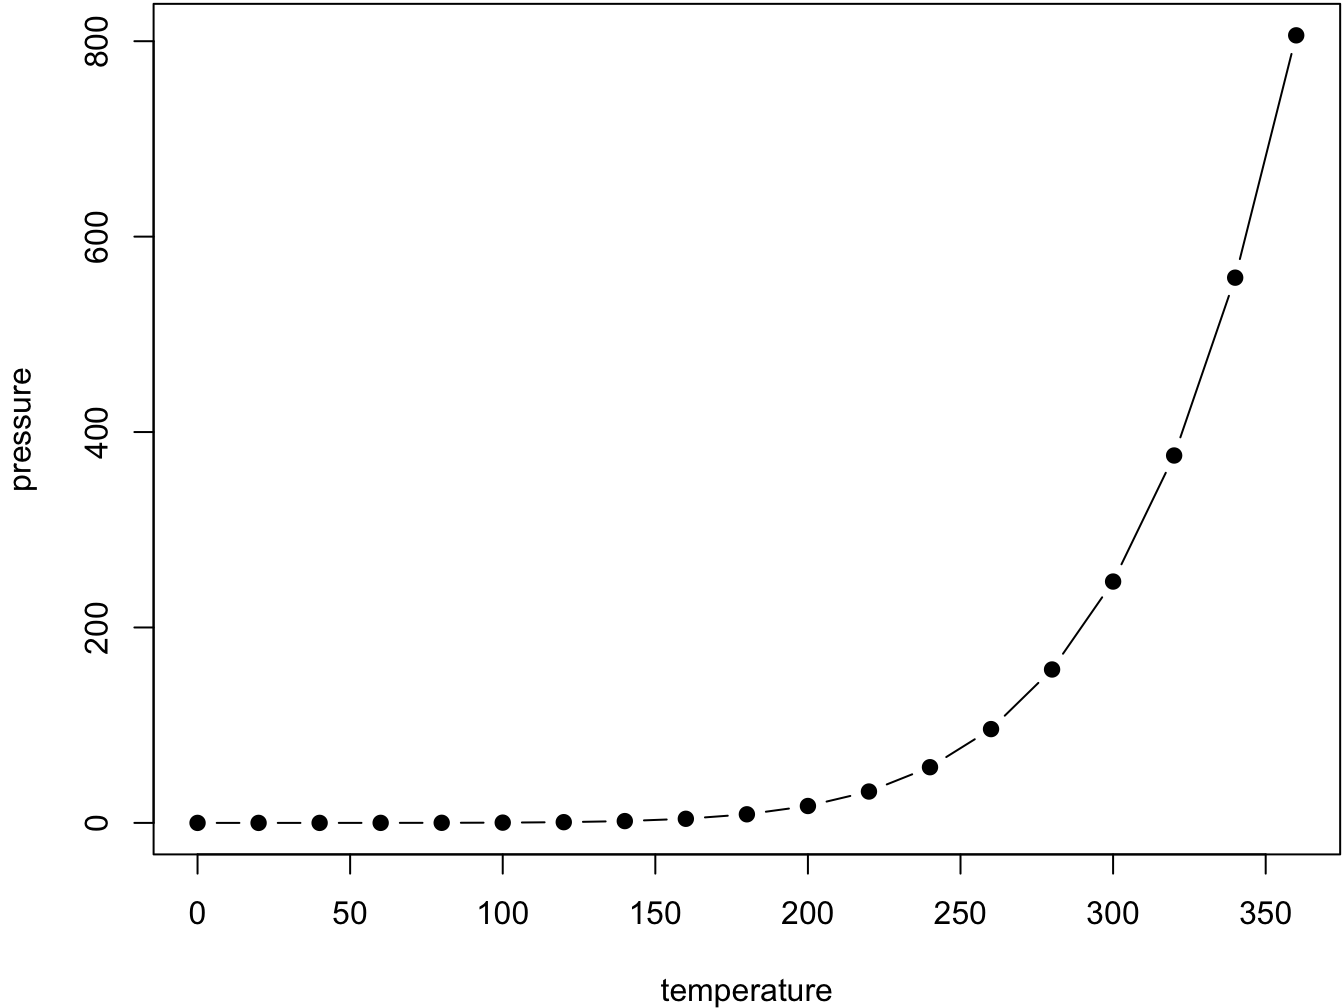
\includegraphics[width=0.8\linewidth]{02-privacy-and-autonomy_files/figure-latex/nice-fig-1} 

}

\caption{Here is a nice figure!}\label{fig:nice-fig}
\end{figure}

Don't miss Table \ref{tab:nice-tab}.

\begin{Shaded}
\begin{Highlighting}[]
\NormalTok{knitr}\SpecialCharTok{::}\FunctionTok{kable}\NormalTok{(}
  \FunctionTok{head}\NormalTok{(pressure, }\DecValTok{10}\NormalTok{), }\AttributeTok{caption =} \StringTok{\textquotesingle{}Here is a nice table!\textquotesingle{}}\NormalTok{,}
  \AttributeTok{booktabs =} \ConstantTok{TRUE}
\NormalTok{)}
\end{Highlighting}
\end{Shaded}

\begin{table}

\caption{\label{tab:nice-tab}Here is a nice table!}
\centering
\begin{tabular}[t]{rr}
\toprule
temperature & pressure\\
\midrule
0 & 0.0002\\
20 & 0.0012\\
40 & 0.0060\\
60 & 0.0300\\
80 & 0.0900\\
\addlinespace
100 & 0.2700\\
120 & 0.7500\\
140 & 1.8500\\
160 & 4.2000\\
180 & 8.8000\\
\bottomrule
\end{tabular}
\end{table}

\hypertarget{ch-fairness}{%
\chapter{Fairness}\label{ch-fairness}}

You can add parts to organize one or more book chapters together. Parts can be inserted at the top of an .Rmd file, before the first-level chapter heading in that same file.

Add a numbered part: \texttt{\#\ (PART)\ Act\ one\ \{-\}} (followed by \texttt{\#\ A\ chapter})

Add an unnumbered part: \texttt{\#\ (PART\textbackslash{}*)\ Act\ one\ \{-\}} (followed by \texttt{\#\ A\ chapter})

Add an appendix as a special kind of un-numbered part: \texttt{\#\ (APPENDIX)\ Other\ stuff\ \{-\}} (followed by \texttt{\#\ A\ chapter}). Chapters in an appendix are prepended with letters instead of numbers.

\hypertarget{ch-alignment-and-control}{%
\chapter{Alignment and Control}\label{ch-alignment-and-control}}

\hypertarget{footnotes}{%
\section{Footnotes}\label{footnotes}}

Footnotes are put inside the square brackets after a caret \texttt{\^{}{[}{]}}. Like this one \footnote{This is a footnote.}.

\hypertarget{citations}{%
\section{Citations}\label{citations}}

Reference items in your bibliography file(s) using \texttt{@key}.

For example, we are using the \textbf{bookdown} package \citep{R-bookdown} (check out the last code chunk in index.Rmd to see how this citation key was added) in this sample book, which was built on top of R Markdown and \textbf{knitr} \citep{xie2015} (this citation was added manually in an external file book.bib).
Note that the \texttt{.bib} files need to be listed in the index.Rmd with the YAML \texttt{bibliography} key.

The \texttt{bs4\_book} theme makes footnotes appear inline when you click on them. In this example book, we added \texttt{csl:\ chicago-fullnote-bibliography.csl} to the \texttt{index.Rmd} YAML, and include the \texttt{.csl} file. To download a new style, we recommend: \url{https://www.zotero.org/styles/}

The RStudio Visual Markdown Editor can also make it easier to insert citations: \url{https://rstudio.github.io/visual-markdown-editing/\#/citations}

\hypertarget{ch-explainability}{%
\chapter{Explainability and Interpretability}\label{ch-explainability}}

\hypertarget{equations}{%
\section{Equations}\label{equations}}

Here is an equation.

\begin{equation} 
  f\left(k\right) = \binom{n}{k} p^k\left(1-p\right)^{n-k}
  \label{eq:binom}
\end{equation}

You may refer to using \texttt{\textbackslash{}@ref(eq:binom)}, like see Equation \eqref{eq:binom}.

\hypertarget{theorems-and-proofs}{%
\section{Theorems and proofs}\label{theorems-and-proofs}}

\begin{theorem}
\protect\hypertarget{thm:tri}{}\label{thm:tri}For a right triangle, if \(c\) denotes the \emph{length} of the hypotenuse
and \(a\) and \(b\) denote the lengths of the \textbf{other} two sides, we have
\[a^2 + b^2 = c^2\]
\end{theorem}

Labeled theorems can be referenced in text using \texttt{\textbackslash{}@ref(thm:tri)}, for example, check out this smart theorem \ref{thm:tri}.

Read more here \url{https://bookdown.org/yihui/bookdown/markdown-extensions-by-bookdown.html}.

\hypertarget{callout-blocks}{%
\section{Callout blocks}\label{callout-blocks}}

The \texttt{bs4\_book} theme also includes special callout blocks, like this \texttt{.rmdnote}.

You can use \textbf{markdown} inside a block.

\begin{Shaded}
\begin{Highlighting}[]
\FunctionTok{head}\NormalTok{(beaver1, }\AttributeTok{n =} \DecValTok{5}\NormalTok{)}
\CommentTok{\#\textgreater{}   day time  temp activ}
\CommentTok{\#\textgreater{} 1 346  840 36.33     0}
\CommentTok{\#\textgreater{} 2 346  850 36.34     0}
\CommentTok{\#\textgreater{} 3 346  900 36.35     0}
\CommentTok{\#\textgreater{} 4 346  910 36.42     0}
\CommentTok{\#\textgreater{} 5 346  920 36.55     0}
\end{Highlighting}
\end{Shaded}

It is up to the user to define the appearance of these blocks for LaTeX output.

You may also use: \texttt{.rmdcaution}, \texttt{.rmdimportant}, \texttt{.rmdtip}, or \texttt{.rmdwarning} as the block name.

The R Markdown Cookbook provides more help on how to use custom blocks to design your own callouts: \url{https://bookdown.org/yihui/rmarkdown-cookbook/custom-blocks.html}

\hypertarget{ch-safety}{%
\chapter{Safety, Security and Accountability}\label{ch-safety}}

\hypertarget{publishing}{%
\section{Publishing}\label{publishing}}

HTML books can be published online, see: \url{https://bookdown.org/yihui/bookdown/publishing.html}

\hypertarget{pages}{%
\section{404 pages}\label{pages}}

By default, users will be directed to a 404 page if they try to access a webpage that cannot be found. If you'd like to customize your 404 page instead of using the default, you may add either a \texttt{\_404.Rmd} or \texttt{\_404.md} file to your project root and use code and/or Markdown syntax.

\hypertarget{metadata-for-sharing}{%
\section{Metadata for sharing}\label{metadata-for-sharing}}

Bookdown HTML books will provide HTML metadata for social sharing on platforms like Twitter, Facebook, and LinkedIn, using information you provide in the \texttt{index.Rmd} YAML. To setup, set the \texttt{url} for your book and the path to your \texttt{cover-image} file. Your book's \texttt{title} and \texttt{description} are also used.

This \texttt{bs4\_book} provides enhanced metadata for social sharing, so that each chapter shared will have a unique description, auto-generated based on the content.

Specify your book's source repository on GitHub as the \texttt{repo} in the \texttt{\_output.yml} file, which allows users to view each chapter's source file or suggest an edit. Read more about the features of this output format here:

\url{https://pkgs.rstudio.com/bookdown/reference/bs4_book.html}

Or use:

\begin{Shaded}
\begin{Highlighting}[]
\NormalTok{?bookdown}\SpecialCharTok{::}\NormalTok{bs4\_book}
\end{Highlighting}
\end{Shaded}

\hypertarget{build-information}{%
\chapter*{Build Information}\label{build-information}}
\addcontentsline{toc}{chapter}{Build Information}

This book was written in \href{http://bookdown.org/}{bookdown} inside \href{http://www.rstudio.com/ide/}{RStudio}. The website \href{https://ethics-1.zakvarty.com}{ethics-1.zakvarty.com} is hosted with \href{https://www.netlify.com}{Netlify}. The complete source is available from \href{https://github.com/zakvarty/ethics-1}{GitHub}.

The \href{assets/ethics-1-logo.png}{course logo} was designed by \href{https://www.zakvarty.com/}{Zak Varty}.

This version of the book was built with:

\begin{verbatim}
#>  setting  value
#>  version  R version 4.2.0 (2022-04-22)
#>  os       macOS Big Sur/Monterey 10.16
#>  system   x86_64, darwin17.0
#>  ui       X11
#>  language (EN)
#>  collate  en_GB.UTF-8
#>  ctype    en_GB.UTF-8
#>  tz       Europe/London
#>  date     2022-07-28
#>  pandoc   2.18 @ /Applications/RStudio.app/Contents/MacOS/quarto/bin/tools/ (via rmarkdown)
\end{verbatim}

Along with these packages:

\begin{tabular}{l|l|l|l}
\hline
Package & Version & Date & Source\\
\hline
bookdown & 0.26 & 2022-04-15 & CRAN (R 4.2.0)\\
\hline
brio & 1.1.3 & 2021-11-30 & CRAN (R 4.2.0)\\
\hline
cachem & 1.0.6 & 2021-08-19 & CRAN (R 4.2.0)\\
\hline
callr & 3.7.0 & 2021-04-20 & CRAN (R 4.2.0)\\
\hline
cli & 3.3.0 & 2022-04-25 & CRAN (R 4.2.0)\\
\hline
crayon & 1.5.1 & 2022-03-26 & CRAN (R 4.2.0)\\
\hline
desc & 1.4.1 & 2022-03-06 & CRAN (R 4.2.0)\\
\hline
devtools & 2.4.3 & 2021-11-30 & CRAN (R 4.2.0)\\
\hline
digest & 0.6.29 & 2021-12-01 & CRAN (R 4.2.0)\\
\hline
ellipsis & 0.3.2 & 2021-04-29 & CRAN (R 4.2.0)\\
\hline
evaluate & 0.15 & 2022-02-18 & CRAN (R 4.2.0)\\
\hline
fastmap & 1.1.0 & 2021-01-25 & CRAN (R 4.2.0)\\
\hline
fs & 1.5.2 & 2021-12-08 & CRAN (R 4.2.0)\\
\hline
glue & 1.6.2 & 2022-02-24 & CRAN (R 4.2.0)\\
\hline
htmltools & 0.5.2 & 2021-08-25 & CRAN (R 4.2.0)\\
\hline
knitr & 1.39 & 2022-04-26 & CRAN (R 4.2.0)\\
\hline
lifecycle & 1.0.1 & 2021-09-24 & CRAN (R 4.2.0)\\
\hline
magrittr & 2.0.3 & 2022-03-30 & CRAN (R 4.2.0)\\
\hline
memoise & 2.0.1 & 2021-11-26 & CRAN (R 4.2.0)\\
\hline
pkgbuild & 1.3.1 & 2021-12-20 & CRAN (R 4.2.0)\\
\hline
pkgload & 1.2.4 & 2021-11-30 & CRAN (R 4.2.0)\\
\hline
prettyunits & 1.1.1 & 2020-01-24 & CRAN (R 4.2.0)\\
\hline
processx & 3.5.3 & 2022-03-25 & CRAN (R 4.2.0)\\
\hline
ps & 1.7.0 & 2022-04-23 & CRAN (R 4.2.0)\\
\hline
purrr & 0.3.4 & 2020-04-17 & CRAN (R 4.2.0)\\
\hline
R6 & 2.5.1 & 2021-08-19 & CRAN (R 4.2.0)\\
\hline
remotes & 2.4.2 & 2021-11-30 & CRAN (R 4.2.0)\\
\hline
rlang & 1.0.2 & 2022-03-04 & CRAN (R 4.2.0)\\
\hline
rmarkdown & 2.14 & 2022-04-25 & CRAN (R 4.2.0)\\
\hline
rprojroot & 2.0.3 & 2022-04-02 & CRAN (R 4.2.0)\\
\hline
rstudioapi & 0.13 & 2020-11-12 & CRAN (R 4.2.0)\\
\hline
sessioninfo & 1.2.2 & 2021-12-06 & CRAN (R 4.2.0)\\
\hline
stringi & 1.7.6 & 2021-11-29 & CRAN (R 4.2.0)\\
\hline
stringr & 1.4.0 & 2019-02-10 & CRAN (R 4.2.0)\\
\hline
testthat & 3.1.4 & 2022-04-26 & CRAN (R 4.2.0)\\
\hline
usethis & 2.1.6 & 2022-05-25 & CRAN (R 4.2.0)\\
\hline
withr & 2.5.0 & 2022-03-03 & CRAN (R 4.2.0)\\
\hline
xfun & 0.31 & 2022-05-10 & CRAN (R 4.2.0)\\
\hline
yaml & 2.3.5 & 2022-02-21 & CRAN (R 4.2.0)\\
\hline
\end{tabular}

  \bibliography{book.bib,packages.bib}

\end{document}
